\chapter{Comparison between the MENP framework and the traditional hypothesis testing framework}
Chapter 4 showed that the MENP framework can be applied to spectrum sensing to achieve the largest probability of detection under any possible probability of false alarm constraints. This chapter conducts a comparison between the MNEP framework and the traditional hypothesis testing framework when applied to energy detector in the presence of two primary signals. Two situations, one assuming the detector has no side information of primary users (for a given time slot, the detector does not know which primary signal could occupy the channel) and the other assuming the detector has perfect side information of primary users (for a given time slot, the detector knows which primary user could occupy the channel), are considered.  
Performance analysis results, which illustrate the performance of both framework, are presented.

\section{Energy Detection with no Side Information}
\subsection{System Model}
We consider a cognitive radio system where the licensed frequency spectrum could be occupied by one of two distinct signals $\{s_A, s_B\}$ or it could be vacant. 
Let $H_0$ denote the hypothesis under which the channel is free, $H_1$ denote the hypothesis under which the channel is occupied by $s_A$ or $s_B$.
Under hypothesis $H_1$, the channel is occupied by signal $s_A$ with probability $q$ and the channel is occupied by signal $s_B$ with probability $1-q$. %However, the value of $q$ is unknown for the detector.   
We are interested to test $H_0$ against $\bar{H}_0$. The block diagram of the system is illustrated in Figure \ref{pic: ch5 diagram}.  

\begin{figure}[!hbp]
\centering
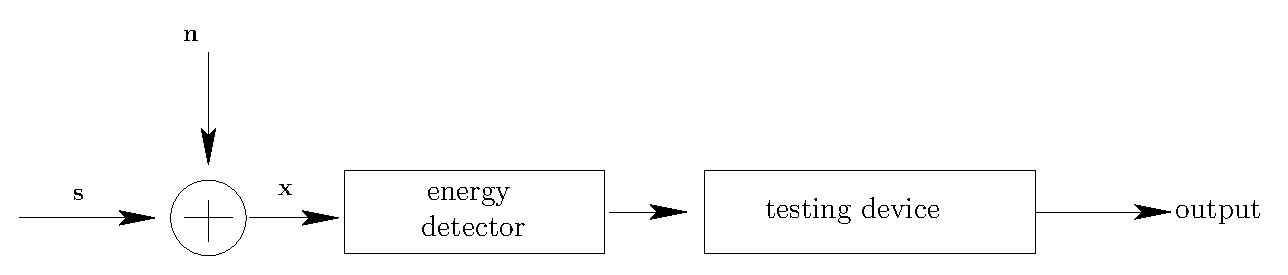
\includegraphics[width = \textwidth]{5/fig4.eps}
\caption{Block Diagram for Energy Detection}
\label{pic: ch5 diagram}
\end{figure}

The detector consists of a measuring device followed by a testing device. The measuring device observes the noises version of the received signals and forms the energy of their sampled version. With this energy, the testing device employs a proper hypothesis testing framework to decide about the state of the channel. We assume during the detection, the channel status does not change. The input to the measuring device can be modeled as 
\begin{eqnarray}
  \mathbf{x} = \begin{cases}
    &\mathbf{n}\;\;\;\;\;\;\text{when $H_0$ is true}\\
    &\mathbf{n} + T\mathbf{s}_A + (1-T)\mathbf{s}_B\;\;\;\;\;\;\text{when $H_1$ is true}
  \end{cases}
  \label{equ:input2energy}
\end{eqnarray}
where
\begin{equation}
  \begin{cases}
	&\mathbf{x} = (x_0, x_1, \cdots, x_{N-1})\\
	&\mathbf{s}_A = (s_{A0}, s_{A1}, \cdots, s_{A(N-1)})\\
	&\mathbf{s}_B = (s_{B0}, s_{B1}, \cdots, s_{B(N-1)})\\
	&\mathbf{n} = (n_{0}, n_{1}, \cdots, n_{N-1})\,,
  \end{cases}
  \label{150621a1}
\end{equation}
and 
\begin{equation}
  T = \begin{cases}
    &0\;\;\;\;\;\;\text{with probability $q$}\\
    &1\;\;\;\;\;\;\text{with probability $1-q$}\,.
  \end{cases}
  \label{150621a2}
\end{equation}

Just like in section 4.1, 
we assume  $s_{A_i}$ $s_{B_i}$ and $n_i$ are zero-mean independent and identically distributed (iid) circularly symmetric complex Gaussian (CSCG) random variables with variances $2\sigma_{s_A}^2$, $2\sigma_{s_B}^2$ and $2\sigma_{n}^2$, i.e., $s_{A_i} \sim \mathcal{CN}(0, 2\sigma_{s_A}^2)$, $s_{B_i} \sim \mathcal{CN}(0, 2\sigma_{s_B}^2)$ and $n_i \sim \mathcal{CN}(0, 2\sigma_{n}^2)$.
Each noisy sample $x_i = s_i + n_i$ is governed by a probability law under each hypothesis. In our model
since the noise and signal are independent, $s_i+ n_i \sim \mathcal{CN}(0, 2(\sigma_{s}^2 + \sigma_n^2))$.  Define $\sigma_0^2 = \sigma_n^2$, $\sigma_1^2 = \sigma_{s_A}^2 + \sigma_n^2$ and $\sigma_2^2 = \sigma_{s_B}^2 + \sigma_n^2$, we can see
\begin{equation}
  \label{1129a1}
  \begin{split}
  n_i &\sim \mathcal{CN}(0, 2\sigma_0^2)\\
  n_i + s_{A_i} &\sim \mathcal{CN}(0, 2\sigma_1^2)\\
   n_i + s_{B_i}&\sim \mathcal{CN}(0, 2\sigma_2^2) \,,
  \end{split}
\end{equation}
thus we have 
\begin{equation}
   \begin{split}
     &\begin{pmatrix} x_{i_R} \\ x_{i_I} \end{pmatrix} \sim \mathcal{N}\Big( \begin{bmatrix} 0 \\ 0 \end{bmatrix}, \begin{bmatrix} \sigma_0^2 & 0\\ 0 & \sigma_0^2 \end{bmatrix} \Big) \text{when no signal is presented}\\
     &\begin{pmatrix} x_{i_R} \\ x_{i_I} \end{pmatrix} \sim \mathcal{N}\Big( \begin{bmatrix} 0 \\ 0 \end{bmatrix}, \begin{bmatrix} \sigma_1^2 & 0\\ 0 & \sigma_1^2 \end{bmatrix} \Big) \text{when $s_A$ is presented}\\
     &\begin{pmatrix} x_{i_R} \\ x_{i_I} \end{pmatrix} \sim \mathcal{N}\Big( \begin{bmatrix} 0 \\ 0 \end{bmatrix}, \begin{bmatrix} \sigma_2^2 & 0\\ 0 & \sigma_2^2 \end{bmatrix} \Big) \text{when $s_B$ is presented}
\end{split}
  \label{equ:xdistribution2}
\end{equation}
where $x_{i_R}$ and $x_{i_I}$ are real and imaginary components of $x_i$. 
Without losing generality, here we assume $\sigma_A^2 < \sigma_B^2$, so we have $\sigma_1^2 < \sigma_2^2$. 
Like in section 4.1, the output of measuring device is
\begin{equation} 
  Y = \sum_{i=0}^{N-1}|x_i|^2 = \sum_{i=0}^{N-1}(x_{i_R}^2+x_{i_I}^2)\,.
  \label{equ: testing device2}
\end{equation}
By observing $y$, a realization of $Y$, the testing device determines the status of the channel. From the analysis in section 3.3 and section 4.1, we know when the channel is ideal, $\frac{Y}{\sigma_0^2} \sim \chi^2(2N)$; when the channel is occupied by signal $s_A$, $\frac{Y}{\sigma_1^2} \sim \chi^2(2N)$; and when the channel is occupied by signal $s_B$, $\frac{Y}{\sigma_2^2} \sim \chi^2(2N)$.  The PDFs and CDFs under each situation are derived in section 3.3 and given as following: 
\def \CHISQUY[#1]{\frac{1}{#1 2^N\Gamma(N)}\left(\frac{y}{#1}\right)^{N-1}\exp\left(-\frac{y}{2#1}\right)}
\begin{equation}
  \begin{split}
   &f_0(y) = \CHISQUY[\sigma_0^2]\\
  &f_1(y|s_A)=  \CHISQUY[\sigma_1^2]\\
  &f_1(y|s_B)=  \CHISQUY[\sigma_2^2]\,;
\end{split}
  \label{20150621a4}
\end{equation} 
and
\begin{equation}
  \begin{split}
    F_0(y) &= F_{\chi^2(2N)}(\frac{y}{\sigma_0^2})\\
    F_1(y|s_A) &= F_{\chi^2(2N)}(\frac{y}{\sigma_1^2})\\
    F_2(y|s_B) &= F_{\chi^2(2N)}(\frac{y}{\sigma_2^2})\,,
  \end{split}
\end{equation}
where $F_{\chi^2(2N)}$ is the CDF of chi-square distribution with $2N$ degrees of freedom. 

From above discussion, we can see under hypothesis $H_1$ the distribution of $Y$ can be written as
\begin{equation}
  \begin{split}
    f_1(y) &= f_1(y|s_A)\text{Pr}(s_A) + f_1(y|s_B)\text{Pr}(s_B)\\
         &= f_1(y|s_A)q + f_1(y|s_B)(1-q)\,,
\end{split}
  \label{20150621a7}
\end{equation}
and thus we have
\begin{equation}
  \begin{split}
    H_0:\;\;\;\;\;&f_0(y) = \CHISQUY[\sigma_0^2]\\
    H_1:\;\;\;\;\;&f_1(y) = q\CHISQUY[\sigma_1^2] + (1-q)\CHISQUY[\sigma_2^2]\,.
  \end{split}
  \label{20150621a8}
\end{equation}

As we can see, $H_0$ is a simple hypothesis and $H_1$ is a composite hypothesis with unknown parameter $p \in [0, 1]$. 
The Neyman Pearson decision rule for \eqref{20150621a8} is
\begin{equation}
  \frac{f_1(y)}{f_0(y)} \substack{H_1 \\ \geq \\ < \\ H_0} \tau\,.
\end{equation}
Substitute $f_0(y)$ and $f_1(y)$ into above equation, we have 
\begin{equation}
  q\left(\frac{\sigma_0^2}{\sigma_1^2}\right)^N\exp\left( (\frac{1}{2\sigma_0^2} -  \frac{1}{2\sigma_1^2}  )y^2 \right)
+ (1-q) \left(\frac{\sigma_0^2}{\sigma_2^2}\right)^N\exp\left( (\frac{1}{2\sigma_0^2} -  \frac{1}{2\sigma_2^2}  )y^2 \right)
\substack{H_1 \\ \geq \\ < \\ H_0} \tau\,.
\label{20150622a0}
\end{equation}
Define 
\begin{equation}
  g(y) = q\left(\frac{\sigma_0^2}{\sigma_1^2}\right)^N\exp\left( (\frac{1}{2\sigma_0^2} -  \frac{1}{2\sigma_1^2}  )y^2 \right)
+ (1-q) \left(\frac{\sigma_0^2}{\sigma_2^2}\right)^N\exp\left( (\frac{1}{2\sigma_0^2} -  \frac{1}{2\sigma_2^2}  )y^2 \right)\,
\end{equation}
and \eqref{20150622a0} can be written as
\begin{equation}
  g(y) \substack{H_1 \\ \geq \\ < \\ H_0} \tau\,.
  \label{20150622a1}
\end{equation}
Since $q, 1-q \geq 0$ and $(\frac{1}{2\sigma_0^2} -  \frac{1}{2\sigma_1^2}  ), (\frac{1}{2\sigma_0^2} -  \frac{1}{2\sigma_2^2}  ) >  0$, we know $g(y)$ is a monotonic increasing function and $g^{-1}(y) $ exists.  
Let $V_\tau = g^{-1}(\tau)$, since $g(y)$ is a monotonic increasing function, we have 
\begin{equation}
  \begin{cases}
    &y > V_\tau\;\;\;\;g(y) > \tau\\
    &y < V_\tau\;\;\;\;g(y) < \tau\,.
  \end{cases}
\end{equation}
Hence \eqref{20150622a1} can be written in form of 
\begin{equation}
  y  \substack{H_1 \\ \geq \\ < \\ H_0} V_\tau\,.
  \label{20150622a2}
\end{equation}

By using decision rule \eqref{20150622a2}, the probability of detection and the probability of false alarm can be written in form of 
\begin{equation}
  \begin{split}
  P_d &= \int_{0}^{V_\tau} f_0(y) \mathrm{d}y = F_0(V_\tau)\\
  P_{f,q} &= \int_{0}^{V_\tau} qf_1(y|s_A) + \int_0^{V_\tau}(1-q)f_1(y|s_B)\mathrm{d}y\\
      &= qF_1(V_\tau|s_A) + (1-q)F_1(V_\tau|s_B)\,.
    \end{split}
    \label{20150622a3}
  \end{equation}
  Here we use $P_{f,q}$ to present the probability of false alarm for a specific $q$.
  As we can see,  $P_{f,q}$ depends on both $V_\tau$ and $q$.   
In the following we will show the UMP test of size $c$ ($c \in (0, 1)$) exists and can be written in form of 
\begin{equation}
\delta^\ast:  y \substack{H_1 \\ \geq \\ < \\ H_0} V_\tau\;\;\;\;\;\;\text{where $F_1(V_\tau|s_A) = c$}\,.
\end{equation}

According to the definition given in \cite{LehmannTest},  $\delta^\ast$ is a UMP test of size $c$ if:
\\(a) for any $q \in [0, 1]$, we have $P_f(\delta^\ast) \leq c$;
\\(b) Assume $\delta'$ is a decision rule satisfy condition (a), we have $P_d(\delta^\ast) \geq P_d(\delta')$.  

First, we will show decision rule $\delta^\ast$ satisfy condition (a). From \eqref{20150622a3}, we have 
\begin{equation}
  \begin{split}
    P_f(\delta^\ast) &= qF_1(V_\tau|s_A) + (1-q)F_1(V_\tau|s_B)\\
    &= qF_1(V_\tau|s_A) + (1-q)F_1(V_\tau|s_A)\\
    &= F_1(V_\tau|s_A) = c\,.
  \end{split}
\end{equation}
Thus we can see for all $q \in [0, 1]$, $P_f \leq c$ is satisfied.

Next we will show for any decision rule $\delta'$ satisfying condition (a), we have $P_d(\delta^\ast) \geq P_d(\delta')$.  
Let $q = 1$, from \eqref{20150622a3} we have 
\begin{equation}
  P_f(\delta^\ast) = F_1(V_\tau|s_A) = c\,.
\end{equation}
Hence we can see for the situation $q=1$,  $\delta^\ast$ is the Neyman Pearson decision rule of size $c$, i.e. when $q=1$, there is no decision rule can achieve a larger $P_d$ while keeping $P_f \leq c$.  

Assume $\delta'$ is a decision rule satisfying condition (a), hence we have when $q = 1$ $P_f(\delta') \leq c$. From above discussion we know $P_d(\delta') \leq P_d(\delta^\ast)$. We can conclude decision rule $\delta^\ast$ also satisfies condition (b). Since decision rule $\delta^\ast$ satisfies both condition (a) and (b), it is the UMP test of size $c$.    
